\documentclass{beamer}
\usetheme{Singapore}

%\usepackage{pstricks,pst-node,pst-tree}
\usepackage{amssymb,latexsym}
\usepackage{graphicx}
\usepackage{fancyvrb}
\usepackage{hyperref}
\usepackage{fancybox}
\usepackage{listings}
\definecolor{codegreen}{rgb}{0,0.6,0}
\definecolor{codegray}{rgb}{0.5,0.5,0.5}
\definecolor{codepurple}{rgb}{0.58,0,0.82}
\definecolor{backcolour}{rgb}{0.95,0.95,0.92}

\lstdefinestyle{mystyle}{
    language=Python,
    backgroundcolor=\color{backcolour},   
    commentstyle=\color{codegreen},
    keywordstyle=\color{magenta},
    numberstyle=\tiny\color{codegray},
    stringstyle=\color{codepurple},
    basicstyle=\ttfamily\footnotesize,
    breakatwhitespace=false,         
    breaklines=true,                 
    captionpos=b,                    
    keepspaces=true,                 
    numbers=left,                    
    numbersep=5pt,                  
    showspaces=false,                
    showstringspaces=false,
    showtabs=false,                  
    tabsize=2,
    escapechar=|
}

\lstset{style=mystyle,language=python}


\newcommand{\bi}{\begin{itemize}}
\newcommand{\li}{\item}
\newcommand{\ei}{\end{itemize}}
\newcommand{\Show}[1]{
\begin{center}
\shadowbox{\begin{minipage}{0.8\textwidth}
          #1
          \end{minipage}}
\end{center}
}


\newcommand{\img}[2]{\centerline{\includegraphics[width=#1\textwidth]{#2}}}

\newcommand{\bfr}[1]{\begin{frame}[fragile]\frametitle{{ #1 }}}
\newcommand{\efr}{\end{frame}}

\newcommand{\cola}{\begin{columns}\begin{column}{0.5\textwidth}}
\newcommand{\colb}{\end{column}\begin{column}{0.5\textwidth}}
\newcommand{\colc}{\end{column}\end{columns}}


\title{Think Python 2e, Chapter 1 Notes}
\author{Geoffrey Matthews}

\begin{document}
\begin{frame}
\maketitle

\end{frame}


\bfr{What is a program?}
\bi
\li A sequence of instructions
that specifies how to perform a computation.
\li Examples:
\bi
\li solve a system of equations
\li search and replace text in a document
\li play a video
\li sharpen an image
\li run a simulation
\ei
\ei

\end{frame}

\bfr{Five kinds of instructions}
\bi
\li Input
\li Output
\li Math
\li Conditional execution
\li Repetition
\ei

\end{frame}

\bfr{Idle}

\bi
\li Shell

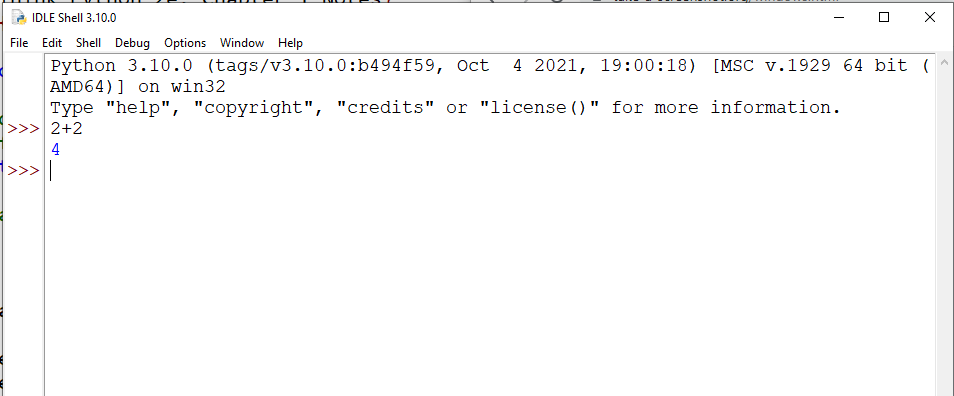
\includegraphics[width=0.8\textwidth]{idleinterpreter}
\li Editor

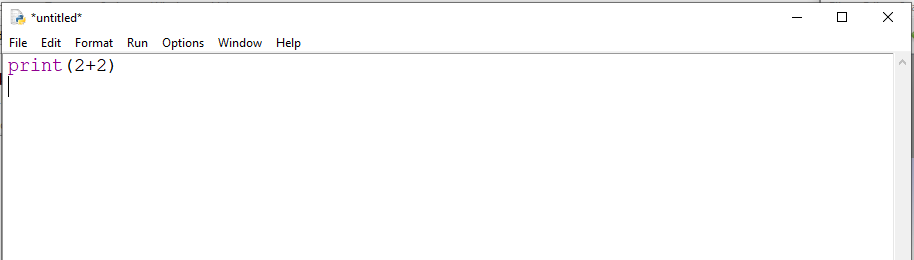
\includegraphics[width=0.8\textwidth]{idleeditor}
\ei

\end{frame}

\bfr{Shell}
\bi
\li Also called {\bf interpreter} or {\bf REPL}

Read-Eval-Print-Loop

\li Great place to learn about Python

\li Not so great for larger programs.
\bi
\li Enter them in the {\bf Editor}
\li Run them: input and output will be in the shell
\ei

\li First program:  \verb|print("Hello world!")|
\bi 
\li Run this in the shell
\li Enter this in the editor, then run module
\ei
\ei

\end{frame}
\bfr{Arithmetic}
\begin{lstlisting}
2 + 2

5 * 5

3 / 4

3 // 4

3 % 4

2 ** 3
\end{lstlisting}

\end{frame}


\bfr{Arithmetic: use parentheses!}
\cola
\begin{lstlisting}

5 - 4 - 3 - 2 - 1

2**3**4

2 + 2/3 + 3

2 * 2/3 * 3
\end{lstlisting}
\pause
\colb

\begin{lstlisting}

((((5 - 4) - 3) - 2) - 1)

2**(3**4)

(2 + 2)/(3 + 3)

(2 * 2)/(3 * 3)
\end{lstlisting}
\colc

\end{frame}

\bfr{Types}
\begin{lstlisting}
type(22)

type(3.14159)

type('hello')

type("hello")

type('22')
\end{lstlisting}

\pause
\vfill

Cats have four legs.
\hfill
``Cats'' has four letters.


\end{frame}

\bfr{Formal languages and natural languages}

\bi
\li {\bf Natural languages:}  English, Spanish, Chinese.
\bi
\li Not designed by people.
\li  Evolved over
thousands of years to serve many purposes.
\li Ambiguous.

\Show{He called her a hacker, and she insulted him.}
\ei
\ei

\end{frame}

\bfr{Formal languages and natural languages}
\bi
\li {\bf Formal languages:} math, chemistry, programming
\bi
\li Designed by people for specific purposes.
\ei

\ei

\Show{Programming languages are formal languages that have been designed to express computations.}

\end{frame}

\bfr{Syntax and Semantics}

Good semantics, bad syntax:

\Show{Me want go store, you takem, kay?}


Good syntax, bad semantics:

\Show{Colorless green ideas sleep furiously.}

\end{frame}

\bfr{Syntax: tokens and structure}

Good structure, bad tokens:

\Show{
This is @ well-structured Engli\$h sentence with invalid t*kens in it. }

Bad structure, good tokens:

\Show{
This sentence all valid tokens has, but invalid structure with.}

\end{frame}

\bfr{Tokens in programming languages.}
\begin{lstlisting}
                 print(333+1756.45)
\end{lstlisting}

\[
\underbrace{\mathtt{print}}_{token}
\underbrace{\mathtt{(}}_{token}
\underbrace{\mathtt{333}}_{token}
\underbrace{\mathtt{+}}_{token}
\underbrace{\mathtt{1756.45}}_{token} 
\underbrace{\mathtt{)}}_{token}
\]


\end{frame}
\bfr{Parsing}

\bi
\li The process of finding the tokens and checking
for correct structure is called {\bf parsing}.
\li
The first task of a computer when processing your
programs is to parse them.
\li Any errors in tokens or structure are
reported back to you as syntax errors.
\li Nothing can be done with a program with syntax errors.
\ei
\pause
\Show{Any homework program submitted with syntax errors
will get zero credit!}

\end{frame}
\bfr{Vocabulary}

\begin{description}
\li[high-level language:]
A programming language like Python that is designed to be easy for humans to read and write.
\li[low-level language:]
A programming language that is designed to be easy for a computer to run; also called “machine language” or “assembly language”.
\li[portability:]
A property of a program that can run on more than one kind of computer.
interpreter:]
A program that reads another program and executes it
\li[prompt:]
Characters displayed by the interpreter to indicate that it is ready to take input from the user.
\li[program:]
A set of instructions that specifies a computation.
\li[print statement:]
An instruction that causes the Python interpreter to display a value on the screen.
\end{description}
\end{frame}
\bfr{Vocabulary}

\begin{description}
\li[operator:]
A special symbol that represents a simple computation like addition, multiplication, or string concatenation.
\li[value:]
One of the basic units of data, like a number or string, that a program manipulates.
\li[type:]
A category of values. The types we have seen so far are integers (type int), floating-point numbers (type float), and strings (type str).
\li[integer:]
A type that represents whole numbers.
\li[floating-point:]
A type that represents numbers with fractional parts.
\li[string:]
A type that represents sequences of characters.
\end{description}
\end{frame}
\bfr{Vocabulary}

\begin{description}
\li[natural language:]
Any one of the languages that people speak that evolved naturally.
\li[formal language:]
Any one of the languages that people have designed for specific purposes, such as representing mathematical ideas or computer programs; all programming languages are formal languages.
\li[token:]
One of the basic elements of the syntactic structure of a program, analogous to a word in a natural language.
\li[syntax:]
The rules that govern the structure of a program.
\li[parse:]
To examine a program and analyze the syntactic structure.
\end{description}

\end{frame}
\end{document}
